\chapter{\IfLanguageName{dutch}{Proof of concept en praktijktest}{Proof of concept and field tests}}
\label{ch:poc}
Na de literatuurstudie, requirementsanalyse en vergelijkende evaluatie van bestaande AI-systemen, vormt dit hoofdstuk een belangrijke schakel in het beantwoorden van de centrale onderzoeksvraag. Hierin wordt het geselecteerde AI-systeem geïmplementeerd in een reële context bij volleybalclub Lindemans Aalst als een proof of concept (PoC).

Deze fase heeft tot doel om de theoretische meerwaarde van het systeem in de praktijk te valideren. Tijdens trainingen en wedstrijden wordt geëvalueerd of het systeem voldoet aan de functionele en technische vereisten zoals geformuleerd in de voorgaande fases. Hierbij wordt bijzondere aandacht besteed aan de gebruiksvriendelijkheid, de nauwkeurigheid van dataverzameling, de snelheid van verwerking en de integratie in de bestaande werkwijze van de club.

Het oorspronkelijke plan voorzag een praktijktestperiode van twee weken. Echter, aangezien het volleybalseizoen onverwacht tot een einde kwam tijdens het midden van deze fase, kon de proof of concept slechts tijdens twee resterende wedstrijden worden uitgevoerd. Ondanks deze beperkte testperiode bood dit toch waardevolle inzichten in de toepasbaarheid en prestaties van het AI-systeem in een wedstrijdcontext.

Door de prestaties van het geautomatiseerde systeem te vergelijken met handmatig geregistreerde gegevens en door feedback van coaches en staf te verzamelen, wordt nagegaan of het AI-systeem daadwerkelijk een significante meerwaarde kan bieden voor de werking van de club. De inzichten uit deze praktijktest vormen een essentiële basis voor het formuleren van aanbevelingen omtrent een bredere implementatie op lange termijn.

\section{Kwartfinale Play-offs - 16/4/2025}
\subsection{Vergelijking van de statistieken}
\subsubsection{Set 1 - Greenyard Maaseik}
\label{sec:PL1_Greenyard1}
% TODO: vergelijking
% TODO: andere stats ook bijzetten 
\begin{figure}
  \centering
  \includegraphics[width=\textwidth]{PL1_AM/SET1/PL1_AM_1.png}
  \caption{\label{fig:PL1_AM_1}Resultaten van de manuele invoer van Greenyard Maaseik in set 1.}
\end{figure}

\begin{table}[ht!]
  \centering
  \scriptsize
  \begin{tabular}{|l|c|c|c|c|c|c|c|c|c|c|c|c|} \hline
    \textbf{Name} & SA & SE & TA & Pct & Eff & Rtg & 0 & 1 & 2 & 3 & ? \\ \hline
    Samuel Fafchamps & 0 & 1 & 3 & 0.67 & -0.33 & 2.33 &  & 1 &  & 2 & 0 \\
    Renet Vancker & 1 & 0 & 2 & 1 & 0.5 & 1.5 & 1 &  &  & 1 & 0 \\
    Thomas Neyens &  &  &  &  &  &  &  &  &  &  &  \\
    Jolan Cox & 0 & 1 & 3 & 0.67 & -0.33 & 2 & 1 & 1 & 1 & 0 &  \\
    Landon Douglas Currie &  &  &  &  &  &  &  &  &  &  &  \\
    Dawid Pawlun & 0 & 1 & 1 & 0 & -1 & 3 &  &  &  & 1 & 0 \\
    Miquel Angel Fornés & 0 & 0 & 4 & 1 & 0 & 1.33 & 2 & 1 &  & 0 &  \\
    Hampus Ekstrand & 0 & 0 & 4 & 1 & 0 & 1 & 3 &  &  & 0 &  \\
    Pierre Perin & 0 & 0 & 3 & 1 & 0 & 1.33 & 2 & 1 &  & 0 &  \\
    Greenyard Maaseik & 1 & 4 & 24 & 0.83 & -0.12 & 2.39 & 1 & 4 & 3 & 15 & 0 \\
    Lindemans Aalst & 1 & 3 & 20 & 0.85 & -0.1 & 1.67 & 1 & 9 & 3 & 5 & 0 \\ \hline
  \end{tabular}
  \caption[Serve statistieken gemaakt door Balltime AI voor Greenyard Maaseik in set 1]{\label{tab:PL1ServeMaaseik1}Serve statistieken gemaakt door Balltime AI voor Greenyard Maaseik in set 1.}
\end{table}

\begin{table}[ht!]
  \centering
  \scriptsize
  \begin{tabular}{|l|c|c|c|c|c|c|c|c|c|} \hline
    \textbf{Name} & 3 & 2 & 1 & 0 & TA & ? & Pass\% & Perfect PP\% & Good GP\% \\ \hline
    Samuel Fafchamps &  &  &  &  &  &  &  &  &  \\
    Renet Vancker &  &  &  &  &  &  &  &  &  \\
    Thomas Neyens & 1 &  & 1 & 0 & 1 & 0 & 0 &  &  \\
    Jolan Cox &  &  &  &  &  &  &  &  &  \\
    Landon Douglas Currie & 4 & 1 & 1 &  & 7 & 1 & 2.5 & 0.67 & 0.83 \\
    Dawid Pawlun &  &  &  &  &  &  &  &  &  \\
    Miquel Angel Fornés &  &  &  &  &  &  &  &  &  \\
    Hampus Ekstrand & 2 & 1 &  & 1 & 4 & 0 & 2 & 0.5 & 0.75 \\
    Pierre Perin & 5 & 1 & 2 &  & 8 & 0 & 2.38 & 0.62 & 0.75 \\
    Greenyard Maaseik & 2 & 3 & 9 &  & 16 & 2 & 1.5 & 0.14 & 0.36 \\
    Lindemans Aalst & 11 & 3 & 4 & 1 & 20 & 1 & 2.26 & 0.58 & 0.74 \\ \hline
  \end{tabular}
  \caption[Receive statistieken gemaakt door Balltime AI voor Greenyard Maaseik in set 1]{\label{tab:PL1ReceiveMaaseik1}Serve statistieken gemaakt door Balltime AI voor Greenyard Maaseik in set 1.}
\end{table}

\begin{table}[ht!]
  \centering
  \scriptsize
  \begin{tabular}{|l|c|c|c|c|c|c|c|}  \hline
    \textbf{Name} & Set Ast & Set TA & Set SE & A/S & PCT & Dig DS & Dig DE \\ \hline
    Samuel Fafchamps &  &  &  &  &  &  &  \\
    Renet Vancker & 4 & 7 & 0 & 4 & 0.57 &  &  \\
    Thomas Neyens & 1 & 0 & 1 & 0 & 0 &  &  \\
    Jolan Cox & 0 & 1 & 0 & 0 & 0 & 1 & 1 \\
    Landon Douglas Currie &  &  &  &  &  &  &  \\
    Dawid Pawlun & 7 & 13 & 0 & 7 & 0.54 & 2 & 0 \\
    Miquel Angel Fornés & 0 & 1 & 0 & 0 & 0 & 1 & 1 \\
    Hampus Ekstrand & 2 & 1 & 1 & 0 & 4 &  &  \\
    Pierre Perin & 0 & 1 & 0 & 1 & 2 &  &  \\
    Greenyard Maaseik & 13 & 21 & 0 & 13 & 0.62 & 7 & 0 \\
    Lindemans Aalst & 11 & 23 & 0 & 11 & 0.5 & 9 & 3 \\ \hline
  \end{tabular}
  \caption[Setting en digging statistieken gemaakt door Balltime AI voor Greenyard Maaseik in set 1]{\label{tab:PL1SetDigMaaseik1}Setting en digging statistieken gemaakt door Balltime AI voor Greenyard Maaseik in set 1.}
\end{table}

\begin{table}[ht!]
  \centering
  \scriptsize
  \begin{tabular}{|l|c|c|c|c|c|c|c|c|c|} \hline
    \textbf{Name} & Attack K & E & TA & Atk\% & Kill\% & K/S & Error\% & Block BS & BA \\ \hline
    Samuel Fafchamps & 3 & 0 & 4 & 0.75 & 0.75 & 3 & 0 &   &   \\
    Renet Vancker &   &   &   &   &   &   &   &   &   \\
    Thomas Neyens &   &   &   &   &   &   &   &   &   \\
    Jolan Cox & 3 & 2 & 6 & 0.17 & 0.5 & 3 & 0.33 & 1 & 0 \\
    Landon Douglas Currie &   &   &   &   &   &   &   &   &   \\
    Dawid Pawlun &   &   &   &   &   &   &   & 1 & 0 \\
    Miquel Angel Fornés & 3 & 0 & 5 & 0.6 & 0.6 & 3 & 0 & 0 & 1 \\
    Hampus Ekstrand & 2 & 1 & 1 & 0 & 0.25 & 1 & 1 & 0 & 0 \\
    Pierre Perin & 1 & 2 & 6 & -0.17 & 0.17 & 1 & 0.33 & 0 & 1 \\
    Greenyard Maaseik & 15 & 4 & 24 & 0.46 & 0.62 & 15 & 0.17 &   &   \\
    Lindemans Aalst & 11 & 4 & 25 & 0.28 & 0.44 & 11 & 0.16 & 2 & 0 \\ \hline
    \end{tabular}
  \caption[Attacking en blocking statistieken gemaakt door Balltime AI voor Greenyard Maaseik in set 1]{\label{tab:PL1AttBlockMaaseik1}Attacking en blocking statistieken gemaakt door Balltime AI voor Greenyard Maaseik in set 1.}
\end{table}

\begin{figure}
  \centering
  \includegraphics[width=\textwidth]{PL1_AM/SET1/ROT_STATS.png}
  \caption{\label{fig:PL1_ROT_STATS_1}Rotatie statistieken gemaakt door Balltime AI voor Greenyard Maaseik in set 1.}
\end{figure}

\subsubsection{Set 2 - Lindemans Aalst}
\label{sec:PL1_Aalst2}
% TODO: vergelijking
% TODO: andere stats ook bijzetten
\begin{figure}
  \centering
  \includegraphics[width=\textwidth]{PL1_AM/SET2/PL1_AM_2.png}
  \caption{\label{fig:PL1_AM_2}Resultaten van de manuele invoer van Lindemans Aalst in set 2.}
\end{figure}

\begin{table}[ht!]
  \centering
  \scriptsize
  \begin{tabular}{|l|c|c|c|c|c|c|c|c|c|c|c|c|} \hline
    \textbf{Name} & SA & SE & TA & Pct & Eff & Rtg & 0 & 1 & 2 & 3 & ? \\ \hline
    Timo Lohmus & 1 & 1 & 4 & 0.75 & 0 & 1.75 & 1 & 2 & 1 & 0 & 1 \\
    Max Schulz & 0 & 1 & 3 & 0.67 & -0.33 & 2.33 &  & 1 &  & 2 & 0 \\
    Hiago Crins & 0 & 0 & 3 & 1 & 0 & 1.67 &  & 2 &  & 1 & 0 \\
    Mihkel Varblane & 0 & 0 & 2 & 1 & 0 & 1 &  & 1 &  &  & 0 \\
    Alvaro Gimeno Rubio & 1 & 1 & 7 & 0.86 & 0 & 1.6 & 1 & 2 &  & 2 & 0 \\
    Robbe Ponseele & 1 & 1 & 2 & 0.5 & 0 & 1.5 & 1 &  &  & 1 & 0 \\
    Lucas Lorente López & 0 & 0 & 3 & 1 & 0 & 2.33 &  & 1 &  & 2 & 0 \\
    Bert Dufraing &  &  &  &  &  &  & 1 &  & 1 &  & 2 \\
    Lindemans Aalst & 0 & 5 & 22 & 0.77 & -0.23 & 2.18 &  & 6 & 6 & 10 & 0 \\
    Greenyard Maaseik & 3 & 4 & 24 & 0.83 & -0.04 & 1.81 & 3 & 7 & 2 & 9 & 0 \\ \hline
  \end{tabular}
  \caption[Serve statistieken gemaakt door Balltime AI voor Lindemans Aalst in set 2]{\label{tab:PL1ServeAalst2}Serve statistieken gemaakt door Balltime AI voor Lindemans Aalst in set 2.}
\end{table}

\begin{table}[ht!]
  \centering
  \scriptsize
  \begin{tabular}{|l|c|c|c|c|c|c|c|c|c|} \hline
    \textbf{Name} & 3 & 2 & 1 & 0 & TA & ? & Pass\% & Perfect PP\% & Good GP\% \\ \hline
    Timo Lohmus & 4 & 3 &  &  & 8 & 0 & 1.75 & 0.12 & 0.62 \\
    Max Schulz & 2 & 2 &  &  & 7 & 0 & 2.14 & 0.43 & 0.71 \\
    Hiago Crins &  &  &  &  &  &  &  &  &  \\
    Mihkel Varblane &  &  &  &  &  &  &  &  &  \\
    Alvaro Gimeno Rubio &  &  &  &  &  &  &  &  &  \\
    Robbe Ponseele &  &  &  &  &  &  &  &  &  \\
    Lucas Lorente López &  &  &  &  &  &  &  &  &  \\
    Bert Dufraing &  &  &  &  &  &  &  &  &  \\
    Lindemans Aalst & 5 & 2 & 7 &  & 17 & 3 & 1.86 & 0.36 & 0.5 \\
    Greenyard Maaseik & 5 & 6 & 6 &  & 17 & 0 & 1.94 & 0.29 & 0.65 \\ \hline
  \end{tabular}
  \caption[Receive statistieken gemaakt door Balltime AI voor Lindemans Aalst in set 2]{\label{tab:PL1ReceiveAalst2}Receive statistieken gemaakt door Balltime AI voor Lindemans Aalst in set 2.}
\end{table}

\begin{table}[ht!]
  \centering
  \scriptsize
  \begin{tabular}{|l|c|c|c|c|c|c|c|} \hline
    \textbf{Name} & Set Ast & Set TA & Set SE & A/S & PCT & Dig DS & Dig DE \\ \hline
    Timo Lohmus & 2 & 0 & 1 & 1 & 2 & 0 & 3 \\
    Max Schulz & 2 & 0 & 1 & 0.5 & 1 & 0 & 5 \\
    Hiago Crins &  &  &  &  &  & 1 & 0 \\
    Mihkel Varblane &  &  &  &  &  & 2 & 0 \\
    Alvaro Gimeno Rubio & 0 & 2 & 0 & 0 & 3 & 0 & 3 \\
    Robbe Ponseele &  &  &  &  &  &  &  \\
    Lucas Lorente López & 10 & 18 & 0 & 10 & 0.56 & 1 & 0 \\
    Bert Dufraing & 1 &  &  &  & 2 & 0 & 2 \\
    Lindemans Aalst & 8 & 23 & 0 & 8 & 0.35 & 6 & 1 \\
    Greenyard Maaseik & 12 & 24 & 0 & 12 & 0.52 & 11 & 0 \\ \hline
  \end{tabular}
  \caption[Setting en digging statistieken gemaakt door Balltime AI voor Lindemans Aalst in set 2]{\label{tab:PL1SetDigAalst2}Setting en digging statistieken gemaakt door Balltime AI voor Lindemans Aalst in set 2.}
\end{table}

\begin{table}[ht!]
  \centering
  \scriptsize
  \begin{tabular}{|l|c|c|c|c|c|c|c|c|c|} \hline
    \textbf{Name} & Attack K & E & TA & Atk\% & Kill\% & K/S & Error\% & Block BS & BA \\ \hline
    Timo Lohmus & 1 & 6 & 0.33 & 0.5 & 0.5 & 0.17 & 0 &  &  \\
    Max Schulz & 3 & 9 & 0.22 & 0.5 & 0.56 & 0.33 & 0 & 4 & 0 \\
    Hiago Crins & 0 & 1 & 0 & 0 & 0 & 0 & 0 & 0 & 2 \\
    Mihkel Varblane & 2 & 0 & 2 & 1 & 1 & 0 & 1 & 2 & 0 \\
    Alvaro Gimeno Rubio & 3 & 2 & 6 & 0.17 & 0.25 & 0.5 & 0.33 & 0 & 1 \\
    Robbe Ponseele &  &  &  &  &  &  &  &  &  \\
    Lucas Lorente López &  &  &  &  &  &  &  & 0 & 1 \\
    Bert Dufraing & 0.5 & 0.5 &  &  &  &  &  &  &  \\
    Lindemans Aalst & 10 & 4 & 26 & 0.23 & 0.33 & 0.09 & 0.38 & 10 & 0.15 \\
    Greenyard Maaseik & 13 & 6 & 24 & 0.29 & 0.47 & 0.54 & 0.25 & 10 & 0 \\ \hline
  \end{tabular}
  \caption[Attacking en blocking statistieken gemaakt door Balltime AI voor Lindemans Aalst in set 2]{\label{tab:PL1AttBlockAalst2}Attacking en blocking statistieken gemaakt door Balltime AI voor Lindemans Aalst in set 2.}
\end{table}

\begin{figure}
  \centering
  \includegraphics[width=\textwidth]{PL1_AM/SET2/ROT_STATS.png}
  \caption{\label{fig:PL1_ROT_STATS_2}Rotatie statistieken gemaakt door Balltime AI voor Lindemans Aalst in set 2.}
\end{figure}

\subsubsection{Set 3 - Greenyard Maaseik}
\label{sec:PL1_Greenyard3}
Voor de opslagen en receptie wordt figuur \ref{fig:PL1ServeMaaseik3} bekeken. 
Het aantal opslagen is bij beide hetzelfde getal. Ook het aantal perfecte (0) opslagen zijn gelijk. De AI-invoer is echter veel minder kritisch dan de manuele invoer. De manuele invoer heeft meer opslagen met score 3, terwijl de AI-invoer meer opslagen heeft met score 1 en 2.

Heel opvallend hier is dat er 8 recepties met score 0 (slechte receptie) zijn bij de manuele invoer en maar 1 bij de AI-invoer. Score 1 werd aan 8 recepties gegeven door de manuele invoer en 10 door de AI. Vijf recepties kregen score 2 door de scouter en zeven recepties kregen diezelfde score door de AI.

\begin{figure}[ht]
\centering
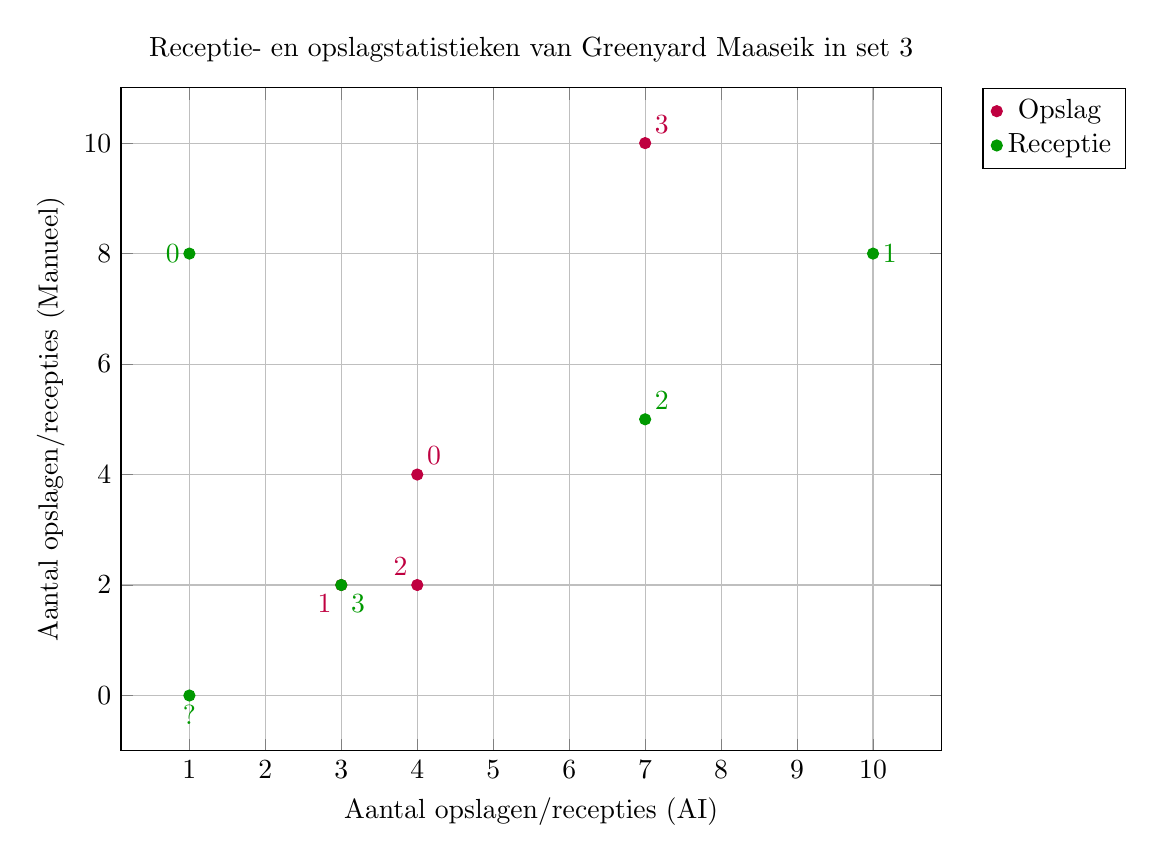
\begin{tikzpicture}
  \begin{axis}[
    title={Receptie- en opslagstatistieken van Greenyard Maaseik in set 3},
    xlabel={Aantal opslagen/recepties (AI)},
    ylabel={Aantal opslagen/recepties (Manueel)},
    grid=major,
    legend style={at={(1.05,1)}, anchor=north west},
    width=12cm,
    height=10cm,
    enlargelimits=0.1,
  ]

  % Opslag (paars)
  \addplot[
    only marks,
    mark=*,
    color=purple,
  ] table {
    x y
    4 4
    3 2
    4 2
    7 10
  };
  \addlegendentry{Opslag}

  % Labels opslag
  \node at (axis cs:4,4) [anchor=south west, purple] {0};
  \node at (axis cs:3,2) [anchor=north east, purple] {1};
  \node at (axis cs:4,2) [anchor=south east, purple] {2};
  \node at (axis cs:7,10) [anchor=south west, purple] {3};

  % Receptie (groen)
  \addplot[
    only marks,
    mark=*,
    color=green!60!black,
  ] table {
    x y
    3 2
    7 5
    10 8
    1 8
    1 0
  };
  \addlegendentry{Receptie}

  % Labels receptie
  \node at (axis cs:3,2) [anchor=north west, green!60!black] {3};
  \node at (axis cs:7,5) [anchor=south west, green!60!black] {2};
  \node at (axis cs:10,8) [anchor=west, green!60!black] {1};
  \node at (axis cs:1,8) [anchor=east, green!60!black] {0};
  \node at (axis cs:1,0) [anchor=north, green!60!black] {?};

  \end{axis}
\end{tikzpicture}
\caption{AI invoer versus manuele invoer, ingedeeld in opslag en receptie, voor Greenyard Maaseik in set 3.}
\label{fig:PL1ServeMaaseik3}
\end{figure}

In tabellen \ref{tab:PL1SetMaaseikMan3} en \ref{tab:PL1SetDigMaaseikAI3} wordt de spelverdeling weergegeven. De hoeveelheden zijn hier zeer verschillend. Bij sommige spelers geeft de manuele invoer ze meer, bij andere dan weer meer door de AI. Volgens manuele invoer heeft Jolan Cox ook vijf keer aan spelverdeling gedaan, terwijl dit door AI geen enkele keer was. Dawid Pawlun heeft door de AI 17 keer aan spelverdeling gedaan, terwijl dit manueel maar 14 keer was. Dit is een verschil van 3. Dit is een groot verschil, maar het kan zijn dat de AI deze als spelverdeling heeft gezien, terwijl dit manueel niet zo was.

Ook bij de verdeding, tabel \ref{tab:PL1DigMaaseikMan3} en \ref{tab:PL1SetDigMaaseikAI3}, zijn er duidelijke verschillen te zien. Hier zijn er ook meerdere spelers die verschillende hoeveelheden verdedigingsacties hebben gekregen. Dit kan iets te maken hebben dat de verdediging buiten het beeld van de camera is gebeurd, waardoor de AI dit niet heeft kunnen registreren.

\begin{table}[ht!]
    \centering
    \scriptsize
    \begin{tabular}{|l|c|c|c|c|c|c|c|c|c|} \hline
        \textbf{Speler} & *E\% & Tot & = & / & - & ! & + & \# \\ \hline
        Samuel Fafchamps  & 100\% & 1 &  &  &  &  & 1 &  \\ 
        Renet Vancker & 100\% & 3 &  &  &  &  & 3 &  \\
        Jolan Cox & 100\% & 5 &  &  &  &  & 5 &  \\ 
        Landon Douglas Currie & 100\% & 1 &  &  &  &  & 1 &  \\ 
        Dawid Pawlun & 100\% & 14 &  &  &  &  & 11 & 3 \\ 
        Hampus Ekstrand & 100\% & 1 &  &  &  &  & 1 &  \\
        Pierre Perin & 100\% & 4 &  &  &  &  & 4 &  \\ \hline
    \end{tabular}
    \caption[Manueel ingevoerde spelverdelingsstatistieken voor Greenyard Maaseik in set 3]{\label{tab:PL1SetMaaseikMan3}Manueel ingevoerde spelverdeling statistieken voor Greenyard Maaseik in set 3.}
\end{table}

\begin{table}[ht!]
    \centering
    \scriptsize
    \begin{tabular}{|l|c|c|c|c|c|c|c|c|c|} \hline
        \textbf{Speler} & *E\% & Tot & = & / & - & ! & + & \#\\ \hline
        Renet Vancker & 0\% & 2 & 1 &  & 1 &  &  &  \\ 
        Jolan Cox & 75\% & 4 &  & 1 & 1 &  & 2 &  \\ 
        Landon Douglas Currie & 50\% & 2 &  &  & 1 &  & 1 &  \\ 
        Dawid Pawlun & 33\% & 3 &  &  & 2 &  & 1 &  \\ 
        Miquel Angel Fornés & 0\% & 2 & 1 &  & 1 &  &  &  \\ 
        Pierre Perin & 67\% & 3 &  &  & 1 &  & 2 &  \\ \hline
    \end{tabular}
    \caption[Manueel ingevoerde verdedigingsstatistieken voor Greenyard Maaseik in set 3]{\label{tab:PL1DigMaaseikMan3}Manueel ingevoerde verdediging statistieken voor Greenyard Maaseik in set 3.}
\end{table}

\begin{table}[ht!]
  \centering
  \scriptsize
  \begin{tabular}{|l|c|c|c|c|c|c|c|} \hline
    \textbf{Speler} & Ast & TA & SE & PCT & DS & DE \\ \hline
    Samuel Fafchamps &  & 1 &  & 0\% &  &  \\
    Renet Vancker &  & 3 &  & 0\% & 1 &  \\
    Jolan Cox &  &  &  &  &  5 &  \\
    Landon Douglas Currie &  & 2 &  & 0\% & 3 & 1 \\
    Dawid Pawlun & 6 & 17 &  & 35\% & 4 &  \\
    Tijmen Bus &  & 1 &  & 0\% & 1 &  \\
    Hampus Ekstrand & 1 & 2 & & 50\% &  &  \\
    Piere Perin &  & 5 &  & 0\% & 2 &  \\  \hline
  \end{tabular}
  \caption[Spelverdelings- en verdedigingsstatistieken gemaakt door Balltime AI voor Greenyard Maaseik in set 3]{\label{tab:PL1SetDigMaaseikAI3}Spelverdelings- en verdedigingsstatistieken gemaakt door Balltime AI voor Greenyard Maaseik in set 3.}
\end{table}

Tabel \ref{tab:PL1AttMaaseikMan3}, \ref{tab:PL1BlockMaaseikMan3} en \ref{tab:PL1AttBlockMaaseikAI3} tonen de de aanval en blokstatistieken gemaakt door de AI en de manuele invoer voor Greenyard Maaseik in set 3. 

De aanvallen worden correct geregisteerd door de AI, behalve bij één speler. Jolan Cox heeft een aanval te minder dan bij de manuele invoer. 

De aanvallen en blokkeringen worden door de AI niet beoordeeld op kwaliteit. Ook worden de blokkeringen op een totaal andere manier bekeken door de AI. Dit systeem geeft geen duidelijke blokpunten. Dit is echter wel van belang.

\begin{table}[ht!]
    \centering
    \scriptsize
    \begin{tabular}{|l|c|c|c|c|c|c|c|c|c|} \hline
        \textbf{Speler} & *E\% & Tot & = & / & - & ! & + & \#\\ \hline
        Andris Sirjakovs & -67\% & 3 &  & 2 &  &  & 1 &  \\ 
        Jolan Cox & 0\% & 5 &  & 1 & 3 &  &  & 1 \\ 
        Dawid Pawlun & 0\% & 2 & 1 &  &  &  &  & 1 \\ 
        Tijmen Bus & -25\% & 4 & 1 & 1 &  & 1 &  & 1 \\ 
        Miquel Angel Fornés & 50\% & 2 &  &  &  &  & 1 & 1 \\ 
        Hampus Ekstrand & 12\% & 8 & 1 & 1 & 1 & 1 & 1 & 3 \\ 
        Pierre Perin  & 17\% & 6 & 1 &  & 2 & 1 &  & 2 \\ \hline
    \end{tabular}
   \caption[Manueel ingevoerde aanvalsstatistieken voor Greenyard Maaseik in set 3]{\label{tab:PL1AttMaaseikMan3}Manueel ingevoerde aanvalsstatistieken voor Greenyard Maaseik in set 3.}
\end{table}

\begin{table}[ht!]
    \centering
    \scriptsize
    \begin{tabular}{|l|c|c|c|c|c|c|c|c|c|} \hline
        \textbf{Speler} & *E\% & Tot & = & / & - & ! & + & \#\\ \hline
        Samuel Fafchamps & 50\% & 2 &  &  &  & 1 &  & 1 \\ 
        Jolan Cox & -100\% & 1 & 1 &  &  &  &  &  \\
        Dawid Pawlun & -25\% & 4 & 1 & 1 &  &  & 1 & 1 \\
        Miquel Angel Fornés & 0\% & 3 & 1 &  &  & 1 &  & 1 \\ 
        Pierre Perin & 0\% & 1 &  &  &  & 1 &  &  \\ \hline
    \end{tabular}
    \caption[Manueel ingevoerde blokstatistieken voor Greenyard Maaseik in set 3]{\label{tab:PL1BlockMaaseikMan3}Manueel ingevoerde blokstatistieken voor Greenyard Maaseik in set 3.}
\end{table}

\begin{table}[ht!]
  \centering
  \scriptsize
  \begin{tabular}{|l|c|c|c|c|c|c|c|c|c|c|c|} \hline
    \textbf{Speler} &  K & E & TA & Atk\% & Kill\% & Error\% & BS & BA & BE \\ \hline
    Samuel Fafchamps &   &   &   &   &   &   & 1 &  & \\
    Andris Sirjakovs &  & 2 & 3 & -0.67 & 0\% & 67\% &   &  & \\
    Jolan Cox & 1 & 1 & 6 & 0.00 & 17\% & 17\% &  &  & \\
    Dawid Pawlun & 1 & 1 & 2 & 0.00 & 50\% & 50\% & 1 &  & \\
    Tijmen Bus &  & 2 & 4 & -0.50 & 0\% & 50\% & &  &  \\
    Miquel Angel Fornés & 1 &  & 2 & 0.50 & 50\% & 0\% & 1 & & \\
    Hampus Ekstrand & 3 & 1 & 8 & 0.25 & 38\% & 12\% &   &   &  \\
    Piere Perin & 2 & 1 & 6 & 0.17 & 33\% & 17 \%&  &  & \\ \hline
  \end{tabular}
  \caption[Aanvals- en blokstatistieken gemaakt door Balltime AI voor Greenyard Maaseik in set 3]{\label{tab:PL1AttBlockMaaseikAI3}Aanvals- en blokstatistieken gemaakt door Balltime AI voor Greenyard Maaseik in set 3.}
\end{table}

\subsection{Vergelijking van de opslagsnelheden}
\label{sec:snelheden}

\begin{table}[h!]
  \centering
  \scriptsize
  \begin{tabular}{|c|c|c|c|} \hline
    L.A.-G.M. & L.A. & G.M. & km/u \\ \hline
    0-0 & 7 & & 97 \\
    1-0 & 7 & & 100 \\
    2-0 & 7 & & 97 \\
    2-1 & & 14 & 43 \\
    3-1 & 1 & & 53 \\
    3-2 & & 10 & 85 \\
    4-2 & 13 & & 95 \\
    4-3 & & 15 & 79 \\
    5-3 & 9 & & 97 \\
    6-3 & 9 & & 100 \\
    6-4 & & 2 & 69 \\
    7-4 & 11 & & 101 \\
    7-5 & & 12 & 92 \\
    8-5 & 14 & & 56 \\
    8-6 & & 19 & 105 \\
    9-6 & 7 & & 63 \\
    9-7 & & 14 & 45 \\
    9-8 & & 14 & 47 \\
    10-8 & 1 & & 58 \\
    10-9 & & 10 & 103 \\
    11-9 & 13 & & 103 \\
    11-10 & & 15 & 95 \\
    11-11 & & 15 & 97 \\
    12-11 & 9 & & 47 \\
    13-11 & 9 & & 97 \\
    13-12 & & 2 & 80 \\
    14-12 & 11 & & 98 \\
    15-12 & 11 & & 56 \\
    16-12 & 11 & & 111 \\
    17-12 & 11 & & 60 \\
    17-13 & & 4 & 58 \\
    18-13 & 14 & & 76 \\
    19-13 & 14 & & 58 \\
    19-14 & & 19 & 103 \\
    19-15 & & 19 & 97 \\
    20-15 & 7 & & 98 \\
    20-16 & & 14 & 53 \\
    21-16 & 3 & & 108 \\
    21-17 & & 10 & 93 \\
    22-17 & 13 & & 100 \\
    23-17 & 13 & & 101 \\
    23-18 & & 15 & 97 \\
    24-18 & 9 & & 100 \\
    24-19 & & 2 & 101 \\
    25-19 & & & \\ \hline
  \end{tabular}
  \caption[Manueel gemeten opslagsnelheden tijdens set 1]{\label{tab:PL1ServeMan1}Manueel gemeten opslagsnelheden tijdens set 1.}
\end{table}

\begin{table}[h!]
  \centering
  \scriptsize
  \begin{tabular}{|c|c|c|c|} \hline
    L.A.-G.M. & L.A. & G.M. & km/u \\ \hline
    0-0 &  & 19 & 116 \\
    1-0 & 7 & & 93 \\
    1-1 &  & 14 & 50 \\
    2-1 & 1 & & 51 \\
    3-1 & 1 & & 53 \\
    3-2 &  & 10 & 95 \\
    4-2 & 13 & & 89 \\
    4-3 &  & 15 & 71 \\
    5-3 & 9 & & 97 \\
    5-4 &  & 2 & 90 \\
    6-4 & 11 & & 82 \\
    6-5 &  & 4 & 61 \\
    7-5 & 14 & & 53 \\
    7-6 &  & 19 & 116 \\
    8-6 & 7 &  & 101 \\
    8-7 &  & 14 & 55 \\
    8-8 &  & 14 & 58 \\
    9-8 & 7 & & 60 \\
    9-9 &  & 10 & 106 \\
    10-9 & 13 & & 80 \\
    11-9 & 13 & & 95 \\
    12-9 & 13 & & 97 \\
    12-10 &  & 15 & 109 \\
    12-11 &  & 15 & 92 \\
    13-11 & 9 &  & 55 \\
    13-12 &  & 2 & 93 \\
    14-12 & 11 &  & 98 \\
    14-13 &  & 4 & 53 \\
    15-13 & 14 &  & 51 \\
    16-13 & 14 &  & 45 \\
    16-14 &  & 19 & 114 \\
    17-14 & 7 &  & 105 \\
    18-14 & 7 &  & 100 \\
    18-15 &  & 14 & 50 \\
    18-16 &  & 14 & 58 \\
    19-16 & 3 &  & 106 \\
    20-16 & 3 &  & 98 \\
    20-17 &  & 10 & 105 \\
    21-17 & 13 &  & 97 \\
    22-17 & 13 &  & 106 \\
    23-17 & 13 &  & 100 \\
    23-18 &  & 15 & 58 \\
    23-19 &  & 15 & 79 \\
    24-19 & 9 &  & 98 \\
    24-20 &  & 2 & 108 \\
    24-21 &  & 2 & 101 \\
    25-21 &  &  &  \\ \hline
  \end{tabular}
  \caption[Manueel gemeten opslagsnelheden tijdens set 2]{\label{tab:PL1ServeMan2}Manueel gemeten opslagsnelheden tijdens set 2.}
\end{table}

\begin{table}[h!]
  \centering
  \scriptsize
  \begin{tabular}{|c|c|c|c|} \hline
    L.A.-G.M. & L.A. & G.M. & km/u \\ \hline
    0-0 & 7 & & 61 \\
    1-0 & 7 & & 89 \\
    2-0 & 7 & & 103 \\
    3-0 & 7 & & 105 \\
    4-0 & 7 & & 108 \\
    5-0 & 7 & & 98 \\
    5-1 & & 14 & 56 \\
    5-2 & & 14 & 53 \\
    6-2 & 1 & & 58 \\
    6-3 & & 10 & 60 \\
    6-4 & & 10 & 103 \\
    7-4 & 13 & & 93 \\
    7-5 &  & 13 & 56 \\
    8-5 & 9 & & 92 \\
    8-6 &  & 2 & 97 \\
    9-6 & 11 & & 60 \\
    10-6 & 11 & & 105 \\
    11-6 & 11 & & 101 \\
    11-7 & & 12 & 84 \\
    12-7 & 14 & & 55 \\
    13-7 & 14 & & 50 \\
    13-8 & & 19 & 100 \\
    13-9 & & 19 & 100 \\
    14-9 & 7 & & 103 \\
    14-10 & & 14 & 56 \\
    15-10 & 1 & & 60 \\
    15-11 & & 10 & 106 \\
    16-11 & 13 & & 98 \\
    17-11 & 13 & & 114 \\
    18-11 & 13 & & 111 \\
    19-11 & 13 & & 113 \\
    20-11 & 13 & & 69 \\
    21-11 & 13 & & 92 \\
    21-12 & & 15 & 76 \\
    21-13 & & 15 & 69 \\
    22-13 & 9 & & 97 \\
    22-14 & & 2 & 69 \\
    22-15 & & 2 & 71 \\
    23-15 & 11 & & 68 \\
    23-16 & & 12 & 84 \\
    24-16 & 14 & & 53 \\
    24-17 & & 19 & 103 \\
    24-18 & & 19 & 101 \\
    25-18 & & & \\ \hline
  \end{tabular}
  \caption[Manueel gemeten opslagsnelheden tijdens set 3]{\label{tab:PL1ServeMan3}Manueel gemeten opslagsnelheden tijdens set 3.}
\end{table}


\section{Kwartfinale Play-offs - 20/4/2025}
\subsection{Vergelijking van de statistieken}
\subsubsection{Set 1 - Greenyard Maaseik}
\label{sec:PL3_Greenyard1}

De opslagstatistieken worden weergeven in tabel \ref{tab:PL3ServeMaaseikMan1} en \ref{tab:PL3ServeMaaseikAI1}. Bij de opslag komt het teken \# overeen met 0, + en / met 1, ! met 2, - en = met 3.
Jolan Cox heeft volgens de AI één opslag meer gegeven dan volgens de manuele invoer. De foutieve opslag van Hampus Ekstrand is wel door beide genoteerd. Opvallend bij deze vergelijking is dat de manuele invoer positiever is bij verschillende opslagen dan de AI.

\begin{table}[ht!]
    \centering
    \scriptsize
    \begin{tabular}{|l|c|c|c|c|c|c|c|c|c|} \hline
        \textbf{Speler} & *E\% & Tot & = & / & - & ! & + & \# \\ \hline
        Samuel Fafchamps & 20\% & 5 &  & & 4 &  & 1 &  \\ 
        Jolan Cox & 100\% & 7 &  & 1 &  & & 6 &  \\ 
        Dawid Pawlun & 50\% & 4 &  &  & 2 & & 2 &  \\
        Miquel Angel Fornés & 33\% & 3 &  & & 2 &  & 1 &  \\
        Hampus Ekstrand & 0\% & 4 & 1 &  & 2 &  & 1 & \\ 
        Pierre Perin & 100\% & 2 &  &  &  & & 2 &  \\ \hline
    \end{tabular}
    \caption[Manueel ingevoerde opslagstatistieken voor Greenyard Maaseik in set 1]{\label{tab:PL3ServeMaaseikMan1}Manueel ingevoerde opslagstatistieken voor Greenyard Maaseik in set 1.}
\end{table}

\begin{table}[ht!]
  \centering
  \scriptsize
  \begin{tabular}{|l|c|c|c|c|c|c|c|c|c|c|c|} \hline
    \textbf{Speler} & SA & SE & TA & Pct & Eff & Rtg & 0 & 1 & 2 & 3 \\ \hline
    Samuel Fafchamps &  &  & 5 & 100 & 0.00 & 2.20 &   & 1 & 2 & 2 \\
    Jolan Cox &  &  & 8 & 100 & 0.00 & 1.67 &   & 3 & 2 & 1 \\
    Dawid Pawlun &  &  & 4 & 100 & 0.00 & 1 .00 &   & 4 &  & 0 \\
    Miquel Angel Fornés &  &  & 3 & 100 & 0.00 & 2.00 &  & 1 & 1 & 1 \\
    Hampus Ekstrand &  & 1 & 4 & 75 & -0.25 & 2.50 &   & & 2 & 2 \\
    Pierre Perin & & & 2 & 100 & 0.00 & 1.00 &   & 1 &   &  \\  \hline
  \end{tabular}
  \caption[Opslagstatistieken gemaakt door Balltime AI voor Greenyard Maaseik in set 1]{\label{tab:PL3ServeMaaseikAI1}Opslagstatistieken gemaakt door Balltime AI voor Greenyard Maaseik in set 1.}
\end{table}

De receptiestatistieken worden weergeven in tabel \ref{tab:PL3ReceiveMaaseikMan1} en  \ref{tab:PL3ReceiveMaaseikAI1}.
De beoordeling van de receptie is op een andere wijze gedaan dan bij de manuele invoer. Bij de manuele invoer wordt er gebruik gemaakt van tekens, terwijl bij de AI-invoer gebruik wordt gemaakt van cijfers. Bij de receptie komt het teken \# overeen met 3, + en / met 2, ! met 1, - en = met 0.
Opmerkelijk is dat Thomas Neyens geen receptie heeft gekregen van de AI, terwijl hij er volgens de manuele invoer wel twee keer receptie heeft genomen. Ook Landon Douglas Currie heeft door AI één receptie minder gekregen dan bij de manuele invoer. Hampus Ekstrand daarentegen heeft dan weer een receptie meer gekregen door de AI. Bij hem is er ook eentje niet beoordeeld kunnen worden. Over het algemeen is de beoordeling tussen de 2 methodes ongeveer gelijk.

\begin{table}[ht!]
    \centering
    \scriptsize
    \begin{tabular}{|l|c|c|c|c|c|c|c|c|c|} \hline
        \textbf{Speler} & *E\% & Tot & = & / & - & ! & + & \# \\ \hline
        Thomas Neyens & -100\% & 2 & 1 & 1 &  &  & & \\
        Landon Douglas Currie & 43\% & 7 & 1 &  & 2 & & 1 & 3 \\ 
        Dawid Pawlun & 0\% & 1 &  &  & 1 &  &  & \\ 
        Hampus Ekstrand & 40\% & 5 &  &  & 1 & 2 & 1 & 1 \\ 
        Pierre Perin & 25\% & 4 & 1 &  & 1 & & 1 & 1 \\ \hline
    \end{tabular}
    \caption[Manueel ingevoerde receptiestatistieken voor Greenyard Maaseik in set 1]{\label{tab:PL3ReceiveMaaseikMan1}Manueel ingevoerde receptiestatistieken voor Greenyard Maaseik in set 1.}
\end{table}

\begin{table}[ht!]
  \centering
  \scriptsize
    \begin{tabular}{|l|c|c|c|c|c|c|c|c|c|} \hline
    \textbf{Speler} & 3 & 2 & 1 & 0 & TA & ? & Pass\% & Perfect PP\% & Good GP\% \\ \hline
    Landon Douglas Currie & 3 & 1 & 2 &   & 6 &  & 2.17 & 5 & 67 \\
    Dawid Pawlun &  &  & 1 &  & 1 &  & 1.00 & 0 & 0 \\
    Hampus Ekstrand & 1 & 2 & 1 & & 5 & 1 & 2.00 & 25 & 75 \\
    Pierre Perin & 2 & 1 &  & 1 & 4 & & 2.00 & 50 & 75 \\  \hline
  \end{tabular}
  \caption[Receptiestatistieken gemaakt door Balltime AI voor Greenyard Maaseik in set 1]{\label{tab:PL3ReceiveMaaseikAI1}Receptiestatistieken gemaakt door Balltime AI voor Greenyard Maaseik in set 1.}
\end{table}

Bij de spelverdelingsstatistieken (door Balltime AI in tabel \ref{tab:PL3SetDigMaaseikAI1}) zijn er bepaalde spelers die een andere hoeveelheid hebben. Sommige hebben één minder, andere dan weer één meer dan bij de manuele invoer, tabel \ref{tab:PL3SetMaaseikMan1}.

Bij de verdedigingsstatistieken (door Balltime AI in tabel \ref{tab:PL3SetDigMaaseikAI1}) zijn er twee speler die volgens de AI wel er verdedinngsactie hebben ondernomen, maar bij de manuele invoer niet. Landon Douglas Currie heeft volgens de AI dan weer één verdeding minder dan bij de manuele invoer, zie tabel \ref{tab:PL3DigMaaseikMan1}.

\begin{table}[ht!]
    \centering
    \scriptsize
    \begin{tabular}{|l|c|c|c|c|c|c|c|c|c|} \hline
        \textbf{Speler} & *E\% & Tot & = & / & - & ! & + & \# \\ \hline
        Jolan Cox & 100\% & 2 &  &  &  &  & 2 &  \\ 
        Dawid Pawlun & 88\% & 17 &  & 1 &  &  & 11 & 5 \\ 
        Miquel Angel Fornés & 100\% & 1 &  &  &  &  & 1 &  \\ 
        Hampus Ekstrand & 100\% & 3 &  &  &  &  & 3 &  \\ \hline
    \end{tabular}
    \caption[Manueel ingevoerde spelverdelingsstatistieken gemaakt voor Greenyard Maaseik in set 1]{\label{tab:PL3SetMaaseikMan1}Manueel ingevoerde spelverdelingsstatistieken gemaakt voor Greenyard Maaseik in set 1.}
\end{table}

\begin{table}[ht!]
    \centering
    \scriptsize
    \begin{tabular}{|l|c|c|c|c|c|c|c|c|c|} \hline
        \textbf{Speler} & *E\% & Tot & = & / & - & ! & + & \# \\ \hline
        Jolan Cox & 100\% & 1 &  & 1 &  &  &  & \\
        Landon Douglas Currie & 25\% & 4 & 2 &  & 1 &  & 1 & \\ 
        Dawid Pawlun & 100\% & 1 &  &  &  &  & 1 & \\
        Pierre Perin & 0\% & 2 &  &  & 2 &  &  &  \\ \hline
    \end{tabular}
    \caption[Manueel ingevoerde verdedigingsstatistieken gemaakt voor Greenyard Maaseik in set 1]{\label{tab:PL3DigMaaseikMan1}Manueel ingevoerde verdedigingsstatistieken gemaakt voor Greenyard Maaseik in set 1.}
\end{table}

\begin{table}[ht!]
  \centering
  \scriptsize
  \begin{tabular}{|l|c|c|c|c|c|c|c|} \hline
    \textbf{Speler} & Ast & TA & SE & A/S & PCT & DS & DE \\ \hline
    Jolan Cox & 1 & 2 &  & 1.00 & 50 & 1 & 0 \\
    Landon Douglas Currie &  &  &  &   &   & 3 &   \\
    Dawid Pawlun & 9 & 16 &  & 9.00 & 60 & 1 & 0 \\
    Miquel Angel Fornés & 1 & 2 &  & 1.00 & 50 & 1 & 1 \\
    Hampus Ekstrand &  & 2 &  & 0.00 & 0 & 1 & \\
    Pierre Perin &   &   &   &   &   & 2 &   \\ \hline
  \end{tabular}
  \caption[Spelverdelings- en verdedigingsstatistieken gemaakt door Balltime AI voor Greenyard Maaseik in set 1]{\label{tab:PL3SetDigMaaseikAI1}Spelverdelings- en verdedigingsstatistieken gemaakt door Balltime AI voor Greenyard Maaseik in set 1.}
\end{table}

Bij de aanvalsstatistieken (door Balltime AI in tabel \ref{tab:PL3AttBlockMaaseikAI1} en manuele invoer in tabel \ref{tab:PL3AttMaaseikMan1}) is er bij één speler een verschillend aantal aanvallen geregistreed. Pierre Perin heeft volgens de AI één keer minder aangevallen dan bij de manuele invoer. Bij de andere spelers is het aantal bij beide hetzelfde. Ook bij deze set zijn de blokstatistieken door de AI, tabel \ref{tab:PL3AttBlockMaaseikAI1}, niet representatief tegen over de manuele invoer, tabel \ref{tab:PL3BlockMaaseikMan1}.

\begin{table}[ht!]
    \centering
    \scriptsize
    \begin{tabular}{|l|c|c|c|c|c|c|c|c|c|} \hline
        \textbf{Speler} & *E\% & Tot & = & / & - & ! & + & \# \\ \hline
        Samuel Fafchamps & 0\% & 2 &  & 1 &  &  &  & 1 \\ 
        Jolan Cox & 20\% & 5 & 1 & 1 &  &  &  & 3 \\ 
        Miquel Angel Fornés & 100\% & 2 &  &  &  &  &  & 2 \\ 
        Hampus Ekstrand & 0\% & 2 &  & 1 &  &  &  & 1 \\ 
        Pierre Perin & 33\% & 12 &  & 2 &  & 2 & 2 & 6 \\ \hline
    \end{tabular}
    \caption[Manueel ingevoerde aanvalsstatistieken gemaakt Greenyard Maaseik in set 1]{\label{tab:PL3AttMaaseikMan1}Manueel ingevoerde aanvalsstatistieken gemaakt voor Greenyard Maaseik in set 1.}
\end{table}

\begin{table}[ht!]
    \centering
    \scriptsize
    \begin{tabular}{|l|c|c|c|c|c|c|c|c|c|} \hline
        \textbf{Speler} & *E\% & Tot & = & / & - & ! & + & \# \\ \hline
        Samuel Fafchamps & -100\% & 2 & 2 &  &  &  &  & \\ 
        Dawid Pawlun & -20\% & 5 & 1 & 1 & 2 & & & 1 \\ 
        Miquel Angel Fornés & -20\% & 5 & 1 & 1 &  & 2 & & 1 \\
        Pierre Perin & 0\% & 1 &  &  & 1 &  &  &\\ \hline
    \end{tabular}
    \caption[Manueel ingevoerde blokstatistieken gemaakt Greenyard Maaseik in set 1]{\label{tab:PL3BlockMaaseikMan1}Manueel ingevoerde blokstatistieken gemaakt voor Greenyard Maaseik in set 1.}
\end{table}

\begin{table}[ht!]
  \centering
  \scriptsize
    \begin{tabular}{|l|c|c|c|c|c|c|c|c|c|c|c|} \hline
    \textbf{Speler} & K & E & TA & Atk\% & Kill\% & K/S & Error\% & BS & BA & BE & B/S \\ \hline
    Samuel Fafchamps & 1 & 1 & 2 & 0.00 & 50 & 1 & 50 &  &  &  & \\
    Jolan Cox & 3 & 2 & 5 & 0.20 & 60 & 3 & 40 &   &  &  &  \\
    Dawid Pawlun &   &   &   &   &   &   &   & 1 & 1 & & 1.00\\
    Miquel Angel Fornés & 2 &  & 2 & 1.00 & 100 & 2 & 0 & 1 & 2 & & 1.00\\
    Hampus Ekstrand & 2 &  & 2 & 1.00 & 100 & 2 & 0 &  & & & \\
    Pierre Perin & 5 & 2 & 11 & 0.27 & 45 & 5 & 18 & 0 & 1 &  & 0.00\\ \hline
  \end{tabular}
  \caption[Aanvals- en blokstatistieken gemaakt door Balltime AI voor Greenyard Maaseik in set 1]{\label{tab:PL3AttBlockMaaseikAI1}Aanvals- en blokstatistieken gemaakt door Balltime AI voor Greenyard Maaseik in set 1.}
\end{table}

\subsubsection{Set 2 - Lindemans Aalst}
\label{sec:PL3_Aalst2}
Figuur \ref{fig:PL3ServeReceiveAalst2} geeft de opslag- en receptiestatistieken weer. 

De perfecte opslagen (0) zijn bij beide hetzelfde aantal weergegeven. Bij de andere opslagen valt op dat de AI meer score 2 geeft en de manuele meer score 1 en 3.

De AI heeft bij één receptie een score van 0 gegeven. Bij de manuele invoer is dit wel het geval voor drie recepties. Ook bij de andere scores wordt duidelijk dat de manuele invoer kritischer is dan de AI. De perfecte recepties (3) zijn wel gelijk. De AI heeft bij één receptie geen score kunnen geven, terwijl de manuele invoer dit wel heeft gedaan. Dit is te zien in de figuur.

\begin{figure}[ht]
\centering
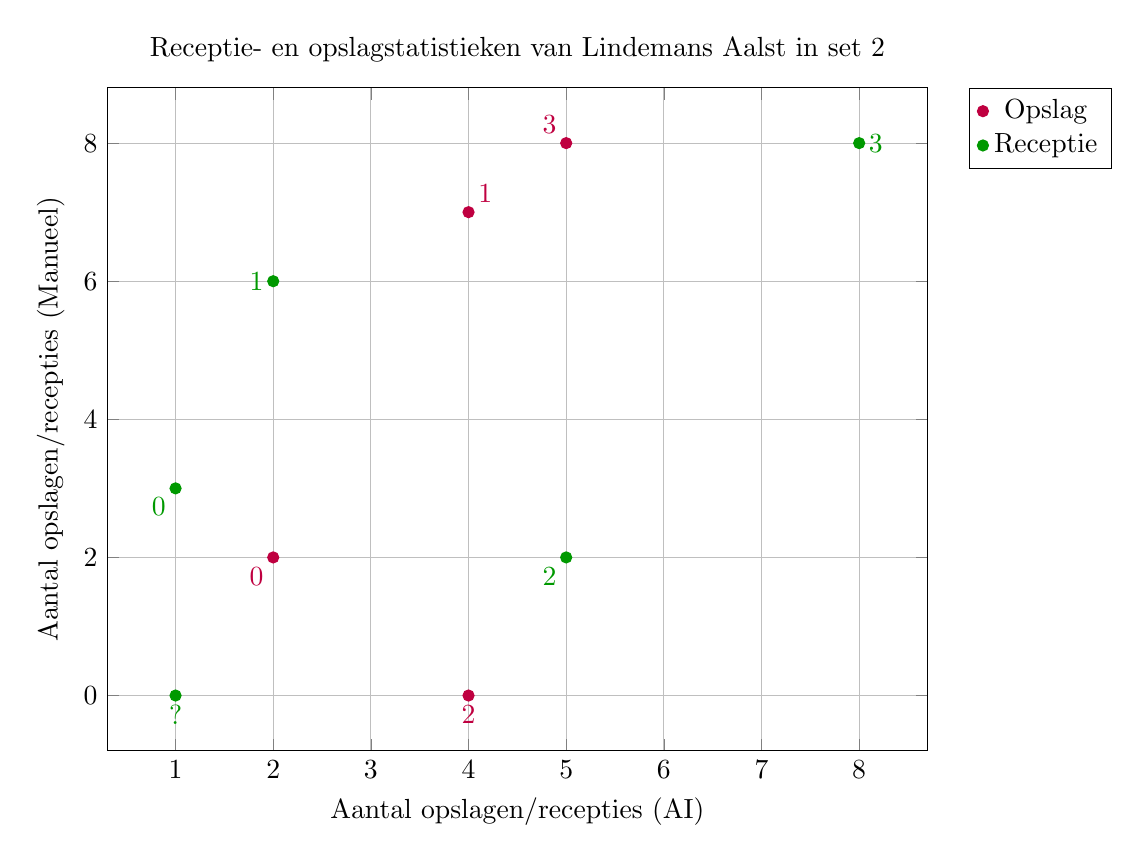
\begin{tikzpicture}
  \begin{axis}[
    title={Receptie- en opslagstatistieken van Lindemans Aalst in set 2},
    xlabel={Aantal opslagen/recepties (AI)},
    ylabel={Aantal opslagen/recepties (Manueel)},
    grid=major,
    legend style={at={(1.05,1)}, anchor=north west},
    width=12cm,
    height=10cm,
    enlargelimits=0.1,
  ]

  % Opslag
  \addplot[
    only marks,
    mark=*,
    color=purple,
  ] table {
    x y
    2 2
    4 7
    4 0
    5 8
  };
  \addlegendentry{Opslag}

  % Labels opslag
  \node at (axis cs:2,2) [anchor=north east, purple] {0};
  \node at (axis cs:4,7) [anchor=south west, purple] {1};
  \node at (axis cs:4,0) [anchor=north, purple] {2};
  \node at (axis cs:5,8) [anchor=south east, purple] {3};

  % Receptie
  \addplot[
    only marks,
    mark=*,
    color=green!60!black,
  ] table {
    x y
    8 8
    5 2
    2 6
    1 3
    1 0
  };
  \addlegendentry{Receptie}

  % Labels receptie
  \node at (axis cs:8,8) [anchor=west, green!60!black] {3};
  \node at (axis cs:5,2) [anchor=north east, green!60!black] {2};
  \node at (axis cs:2,6) [anchor=east, green!60!black] {1};
  \node at (axis cs:1,3) [anchor=north east, green!60!black] {0};
  \node at (axis cs:1,0) [anchor=north, green!60!black] {?};

  \end{axis}
\end{tikzpicture}
\caption{AI invoer versus manuele invoer, ingedeeld in opslag en receptie, voor Lindemans Aalst in set 2.}
\label{fig:PL3ServeReceiveAalst2}
\end{figure}

In tabel \ref{tab:PL3SetAalstMan2} en \ref{tab:PL3DigAalstMan2} zijn de manueel ingevoerde spelverdelings- en verdedigingsstatistieken weergegeven. In tabel \ref{tab:PL3SetDigAalstAI2} zijn dezelfde gegevens weergegeven die door Balltime AI zijn gemaakt.

Het aantal spelverdelingen is bij beide invoermethoden gelijk. Het aantal verdedigingsstatistieken is opnieuw minder bij de AI-invoer tegenover de manuele invoer.

\begin{table}[ht!]
    \centering
    \scriptsize
    \begin{tabular}{|l|c|c|c|c|c|c|c|c|c|}
        \hline
        \textbf{Speler} & *E\% & Tot & = & / & - & ! & + & \# \\ \hline
        Bert Dufraing & 100\% & 1 &  &  & &  & 1 & \\ 
        Lucas Lorente Lòpez & 100\% & 20 &  &  & & & 17 & 3 \\ 
        Matis Verwimp & 100\% & 1 & & & & & 1 & \\ \hline
    \end{tabular}
    \caption[Manueel ingevoerde spelverdelingsstatistieken voor Lindemans Aalst in set 2]{\label{tab:PL3SetAalstMan2}Manueel ingevoerde spelverdelingsstatistieken voor Lindemans Aalst in set 2.}
\end{table}

\begin{table}[ht!]
    \centering
    \scriptsize
    \begin{tabular}{|l|c|c|c|c|c|c|c|c|c|}
        \hline
        \textbf{Speler} & *E\% & Tot & = & / & - & ! & + & \# \\ \hline
        Bert Dufraing & 0\% & 1 & 1 &  &  &  &  & \\ 
        Timo Lohmus & 100\% & 1 &  &  &  &  & 1 & \\ 
        Berre Peters & 67\% & 3 & 1 &  &  &  & 2 & \\ 
        Alvaro Gimeno Rubio & 0\% & 2 & 2 &  &  &  &  & \\ 
        Lucas Lorente Lòpez & 0\% & 1 &  &  & 1 &  &  & \\ 
        Matis Verwimp & 0\% & 1 & 1 & & & & & \\\hline
    \end{tabular}
    \caption[Manueel ingevoerde verdedigingsstatistieken voor Lindemans Aalst in set 2]{\label{tab:PL3DigAalstMan2}Manueel ingevoerde verdedigingsstatistieken voor Lindemans Aalst in set 2.}
\end{table}

\begin{table}[ht!]
  \centering
  \scriptsize
  \begin{tabular}{|l|c|c|c|c|c|c|c|} \hline
    \textbf{Speler} & Ast & TA & SE & PCT & DS & DE \\ \hline
    Bert Dufraing &  & 1 &  & 0\% &  &  \\
    Timo Lohmus &   &   &   &   & 1  &   \\
    Berre Peters &   &   &   &   &  2 &   \\
    Alvaro Gimeno Rubio &  &  &  &  & 1 &   \\
    Lucas Lorente López & 8 & 20 &  & 40\% & 2 &  \\
    Matis Verwimp & 1 & 1 &  & 100\% &   &   \\ \hline
  \end{tabular}
  \caption[Spelverdelings- en verdedigingsstatistieken gemaakt door Balltime AI voor Lindemans Aalst in set 2]{\label{tab:PL3SetDigAalstAI2}Spelverdelings- en verdedigingsstatistieken gemaakt door Balltime AI voor Lindemans Aalst in set 2.}
\end{table}

Bij de aanvalsstatistieken (door Balltime AI in tabel \ref{tab:PL3AttBlockAalstAI2} en manuele invoer in tabel \ref{tab:PL3AttAalstMan2}) is er bij één speler een verschillend aantal aanvallen geregistreerd. Hiago Crins is heeft door de AI twee keer aangevallen, terwijl hij manueel gezien maar één keer heeft aangevallen.

De blokstatistieken (door Balltime AI in tabel \ref{tab:PL3AttBlockAalstAI2} en manuele invoer in tabel \ref{tab:PL3BlockAalstMan2}) zijn ook verschillend. De AI heeft twee aanvallen geregistreerd, terwijl er manueel zes aanvallen zijn geregistreerd. 

\begin{table}[ht!]
    \centering
    \scriptsize
    \begin{tabular}{|l|c|c|c|c|c|c|c|c|c|}
        \hline
        \textbf{Speler} & *E\% & Tot & = & / & - & ! & + & \# \\ \hline
        Hiago Crins & 0\% & 1 &  &  &  & 1 &  & \\ 
        Timo Lohmus & 0\% & 5 &  & 2 & 1 &  & & 2 \\ 
        Berre Peters & 100\% & 2 &  &  & & & & 2 \\ 
        Max Schulz & -25\% & 4 &  & 1 & 1 &  & 2 & \\ 
        Alvaro Gimeno Rubio & 20\% & 5 & 1 & 1 &  &  &  & 3 \\ 
        Lou Kindt & 25\% & 4 &  &  &  &  & 3 & 1 \\
        Lucas Lorente Lòpez & 0\% & 1 &  &  &  & 1 &  & \\ \hline
    \end{tabular}
    \caption[Manueel ingevoerde aanvalsstatistieken voor Lindemans Aalst in set 2]{\label{tab:PL3AttAalstMan2}Manueel ingevoerde aanvalsstatistieken voor Lindemans Aalst in set 2.}
\end{table}

\begin{table}[ht!]
    \centering
    \scriptsize
    \begin{tabular}{|l|c|c|c|c|c|c|c|c|c|}
        \hline
        \textbf{Speler} & *E\% & Tot & = & / & - & ! & + & \# \\ \hline
        Hiago Crins & -50\% & 2 & 1 &  &  &  & 1 &  \\
        Max Schulz & -100\% & 1 & 1 &  &  &  &  & \\
        Mihkel Varblane & -50\% & 2 & 1 &  &  & 1 &  & \\
        Lou Kindt & -100\% & 1 & 1 &  &  &  &  & \\
        Lucas Lorente Lòpez & 0\% & 1 &  &  &  &  & 1 & \\ \hline
    \end{tabular}
    \caption[Manueel ingevoerde blokstatistieken voor Lindemans Aalst in set 2]{\label{tab:PL3BlockAalstMan2}Manueel ingevoerde blokstatistieken voor Lindemans Aalst in set 2.}
\end{table}

\begin{table}[ht!]
  \centering
  \scriptsize
  \begin{tabular}{|l|c|c|c|c|c|c|c|c|c|c|c|} \hline
    \textbf{Speler} &  K & E & TA & Atk\% & Kill\% & Error\% & BS & BA & BE \\ \hline
    Hiago Crins &  &  & 2 & 0.00 & 0\% & 0\% &  &  &\\
    Timo Lohmus & 2 & 2 & 5 & 0.0 & 40\% & 40 \%&  & 1 & \\
    Berre Peters & 2 &  & 2 & 1.00 & 100\% & 0\% &   &  & \\
    Max Schulz & 1 &  & 4 & 0.25 & 25\% & 0\% &   &  & \\
    Mihkel Varblane &   &   &   &   &   &   &  & 1 &\\
    Alvaro Gimeno Rubio & 3 & 2 & 5 & 0.20 & 60\% & 40\% &   &  & \\
    Lou Kindt & 1 &  & 4 & 0.25 & 25\% & 0\% &   &  & \\ \hline
  \end{tabular}
  \caption[Aanvals- en blokstatistieken gemaakt door Balltime AI voor Lindemans Aalst in set 2]{\label{tab:PL3AttBlockAalstAI2}Aanvals- en blokstatistieken gemaakt door Balltime AI voor Lindemans Aalst in set 2.}
\end{table}

\subsubsection{Set 3 - Greenyard Maaseik}
\label{sec:PL3_Greenyard3}
Bij de opslag komt het teken \# overeen met 0, + en / met 1, ! met 2, - en = met 3.

Bij deze tabelen \ref{tab:PL3ReceiveMaaseikMan3} en \ref{tab:PL3ReceiveMaaseikAI3} zijn de receptiestatistieken weergegeven. Hier zijn het totaal aantal opslagen én perfecte opslagen gelijk. Bij de andere scores zijn de opslagen ongeveer gelijk verdeeld.

\begin{table}[ht!]
    \centering
    \scriptsize
    \begin{tabular}{|l|c|c|c|c|c|c|c|c|c|} \hline
        \textbf{Speler} & *E\% & Tot & = & / & - & ! & + & \#\\ \hline
        Samuel Fafchamps & 0\% & 3 &  &  & 3 &  &  &  \\ 
        Renet Vancker & 0\% & 1 &  &  & 1 &  &  & \\ 
        Jolan Cox & 25\% & 4 &  &  & 3 &  &  & 1 \\ 
        Dawid Pawlun & 50\% & 2 &  &  & 1 &  & 1 &  \\ 
        Miquel Angel Fornés & 25\% & 4 &  &  & 3 &  & 1 &  \\ 
        Hampus Ekstrand & 50\% & 4 & 1 &  &  &  & 2 & 1 \\ 
        Pierre Perin & 0\% & 2 & 1 &  &  &  & 1 &  \\ \hline
    \end{tabular}
    \caption[Manueel ingevoerde opslagstatistieken voor Greenyard Maaseik in set 3]{\label{tab:PL3ServeMaaseikMan3}Manueel ingevoerde opslagstatistieken voor Greenyard Maaseik in set 3.}
\end{table}

\begin{table}[ht!]
  \centering
  \scriptsize
  \begin{tabular}{|l|c|c|c|c|c|c|c|c|c|c|c|} \hline
    \textbf{Speler} & SA & SE & TA & Pct & Eff & Rtg & 0 & 1 & 2 & 3 \\ \hline
    Samuel Fafchamps &  &  & 3 & 100\% & 0.00 & 2.67 &   &  & 1 & 2  \\
    Renet Vancker &  &  & 1 & 100\% & 0.00 & 3.00 &  &  &  & 1 \\
    Jolan Cox & 1 &  & 4 & 100\% & 0.25 & 1.50 & 1 & 1 & 1 & 1 \\
    Dawid Pawlun &  &  & 2 & 100\% & 0.00 & 3.00 &   &   & & 1 \\
    Miquel Angel Fornés & 1 & 1 & 4 & 75\% & 0.00 & 2.00 &   & 1 & 2 & 1 \\
    Hampus Ekstrand & 1 & 1 & 4 & 75\% & 0.00 & 1.50 & 1 & 1 & 1 & 1\\
    Pierre Perin & & 1 & 2 & 50\% & -0.50 & 2.5 &   &  & 1 & 1 \\ \hline
  \end{tabular}
  \caption[Opslagstatistieken gemaakt door Balltime AI voor Greenyard Maaseik in set 3]{\label{tab:PL3ServeMaaseikAI3}Opslag statistieken gemaakt door Balltime AI voor Greenyard Maaseik in set 3.}
\end{table}

De beoordeling van de receptie is op een andere wijze gedaan dan bij de manuele invoer. Bij de manuele invoer wordt er gebruik gemaakt van tekens, terwijl bij de AI-invoer gebruik wordt gemaakt van cijfers. Bij de receptie komt het teken \# overeen met 3, + en / met 2, ! met 1, - en = met 0.

Bij deze statistieken (tabellen \ref{tab:PL3ReceiveMaaseikMan3} en \ref{tab:PL3ReceiveMaaseikAI3}) kan geconstateerd worden dat de AI-invoer bepaalde spelers niet heeft geregisteerd. Aan één speler heeft de AI ook een receptie meer gegeven dan de manuele invoer. Opmerkelijk is wel dat de manuele invoer hier voor bepaalde recepties positiever is. Er zijn meer opslagen met een score 3 bij de manuele invoer dan bij de AI.

\begin{table}[ht!]
    \centering
    \scriptsize
    \begin{tabular}{|l|c|c|c|c|c|c|c|c|c|} \hline
        \textbf{Speler} & *E\% & Tot & = & / & - & ! & + & \#\\ \hline
        Jolan Cox & -100\% & 1 & 1 &  &  &  &  & \\ 
        Landon Douglas Currie & 62\% & 8 &  &  & 1 & 2 & 1 & 4 \\ 
        Dawid Pawlun & -100\% & 1 &  & 1 &  &  &  &  \\ 
        Hampus Ekstrand & 100\% & 2 &  &  &  &  & 1 & 1 \\ 
        Pierre Perin & 38\% & 8 & 2 &  & 1 &  & 1 & 4 \\ \hline
    \end{tabular}
    \caption[Manueel ingevoerde receptiestatistieken voor Greenyard Maaseik in set 3]{\label{tab:PL3ReceiveMaaseikMan3}Manueel ingevoerde receptiestatistieken voor Greenyard Maaseik in set 3.}
\end{table}

\begin{table}[ht!]
  \centering
  \scriptsize
  \begin{tabular}{|l|c|c|c|c|c|c|c|c|c|} \hline
    \textbf{Speler} & 3 & 2 & 1 & 0 & TA & Pass\% & PP\% & GP\% \\ \hline
    Landon Douglas Currie & 3 & 3 & 2 &  & 8 & 2.12 & 38\% & 75\% \\
    Hampus Ekstrand & 1 & 1 &   & 2 & & 1.5 & 0\% & 50\% \\
    Pierre Perin & 6 & 1 &   & 2 & 9 & 2.22 & 67\% & 78\% \\ \hline
  \end{tabular}
  \caption[Receptiestatistieken gemaakt door Balltime AI voor Greenyard Maaseik in set 3]{\label{tab:PL3ReceiveMaaseikAI3}Receptiestatistieken gemaakt door Balltime AI voor Greenyard Maaseik in set 3.}
\end{table}

De spelverdelingsstatistieken zijn te vinden in tabel \ref{tab:PL3SetMaaseikMan3} en \ref{tab:PL3SetDigMaaseikAI3}. Die van de verdeding zijn dan weer te vinden in tabel \ref{tab:PL3DigMaaseikMan3} en \ref{tab:PL3SetDigMaaseikAI3}. 

Enkel één speler heeft een verschillend totaal aantal spelverdedingsacties. Bij de manuele invoer heeft hij er géén gedaan, terwijl hij er bij de AI-invoer één heeft gedaan. 

Bij de verdedigingsstatistieken ontbreken er bij de AI-invoer enkele spelers of hebben ze minder ondernomen. 

\begin{table}[ht!]
    \centering
    \scriptsize
    \begin{tabular}{|l|c|c|c|c|c|c|c|c|c|} \hline
        \textbf{Speler} & *E\% & Tot & = & / & - & ! & + & \#\\ \hline
        Renet Vancker & 100\% & 3 &  &  &  &  & 2 & 1 \\ 
        Dawid Pawlun & 100\% & 17 &  &  &  &  & 15 & 2 \\ 
        Pierre Perin & 100\% & 2 &  &  &  &  & 2 &  \\ \hline
    \end{tabular}
    \caption[Manueel ingevoerde spelverdelingsstatistieken voor Greenyard Maaseik in set 3]{\label{tab:PL3SetMaaseikMan3}Manueel ingevoerde spelverdelingsstatistieken voor Greenyard Maaseik in set 3.}
\end{table}

\begin{table}[ht!]
    \centering
    \scriptsize
    \begin{tabular}{|l|c|c|c|c|c|c|c|c|c|} \hline
        \textbf{Speler} & *E\% & Tot & = & / & - & ! & + & \#\\ \hline
        Samuel Fafchamps & 0\% & 1 & 1 &  &  &  &  &  \\ 
        Jolan Cox & 50\% & 2 & 1 & 1 &  &  &  & \\
        Landon Douglas Currie & 33\% & 3 & 1 &  & 1 &  & 1 &  \\
        Dawid Pawlun & 0\% & 3 & 2 &  & 1 &  &  &  \\ 
        Hampus Ekstrand & 100\% & 1 &  &  &  &  & 1 &\\ 
        Pierre Perin & 100\% & 1 &  &  &  &  & 1 & \\ \hline
    \end{tabular}
    \caption[Manueel ingevoerde verdedigingsstatistieken voor Greenyard Maaseik in set 3]{\label{tab:PL3DigMaaseikMan3}Manueel ingevoerde verdedigingsstatistieken voor Greenyard Maaseik in set 3.}
\end{table}

\begin{table}[ht!]
  \centering
  \scriptsize
    \begin{tabular}{|l|c|c|c|c|c|c|c|} \hline
    \textbf{Speler} & Ast & TA & SE & PCT & DS & DE \\ \hline
    Renet Vancker & 2 & 3 &  & 67\% &   &   \\
    Landon Douglas Currie &  & 1 &  & 0\% & 2 & 1 \\
    Dawid Pawlun & 8 & 17 & & 47\% & 2 &  \\
    Hampus Ekstrand &  &  &  &  & 3 &  \\
    Pierre Perin &  & 2 &  & 0\% & 1 &  \\ \hline
  \end{tabular}
  \caption[Spelverdelings- en verdedigingsstatistieken gemaakt door Balltime AI voor Greenyard Maaseik in set 3]{\label{tab:PL3SetDigMaaseikAI3}Spelverdelings- en verdedigingsstatistieken gemaakt door Balltime AI voor Greenyard Maaseik in set 3.}
\end{table}

In tabellen \ref{tab:PL3AttMaaseikMan3} en \ref{tab:PL3BlockMaaseikMan3} zijn de manueel ingevoerde aanvals- en blokstatistieken weergegeven. In tabel \ref{tab:PL3AttBlockMaaseikAI3} zijn de aanvals- en blokstatistieken weergegeven die door Balltime AI zijn gemaakt. 

Het aantal aanvallen is bij beide hetzelfde, behalve bij één speler. Hij heeft een aanval meer bij de AI-invoer. De foutieve aanvallen zijn wel verschillend bij beide. Bij de aanval met de AI-invoer valt op dat Alex Saaremaa een aanval heeft gedaan, wanneer er de beelden worden bekeken is er eigenlijk geen aanval te zien. De AI dacht dat hij een aanval deed, maar eigenlijk is de bal langs hem heen gegaan.

Bij de blokkeringen is er een zeer groot verschil. Bij de AI-invoer zijn er maar twee geweest in de hele set. Terwijl er bij de manuelen invoer dertien blokkeringen zijn geteld.

\begin{table}[ht!]
    \centering
    \scriptsize
    \begin{tabular}{|l|c|c|c|c|c|c|c|c|c|} \hline
        \textbf{Speler} & *E\% & Tot & = & / & - & ! & + & \#\\ \hline
        Samuel Fafchamps & 100\% & 1 &  &  &  &  &  & 1 \\ 
        Jolan Cox & 33\% & 12 &  & 2 &  & 1 & 3 & 6 \\ 
        Miquel Angel Fornés & 33\% & 3 &  & 1 &  &  &  & 2 \\ 
        Hampus Ekstrand & -50\% & 2 & 1 &  &  &  & 1 & \\ 
        Pierre Perin & -50\% & 4 & 3 &  &  &  &  & 1 \\ \hline
    \end{tabular}
    \caption[Manueel ingevoerde aanvalsstatistieken voor Greenyard Maaseik in set 3]{\label{tab:PL3AttMaaseikMan3}Manueel ingevoerde aanvalsstatistieken voor Greenyard Maaseik in set 3.}
\end{table}

\begin{table}[ht!]
    \centering
    \scriptsize
    \begin{tabular}{|l|c|c|c|c|c|c|c|c|c|} \hline
        \textbf{Speler} & *E\% & Tot & = & / & - & ! & + & \#\\ \hline
        Samuel Fafchamps & 33\% & 3 &  &  &  & 1 & 1 & 1 \\ 
        Jolan Cox & -75\% & 4 & 3 &  &  & 1 &  & \\ 
        Dawid Pawlun & -33\% & 3 & 1 &  & 1 & 1 &  &  \\ 
        Miquel Angel Fornés & -100\% & 1 & 1 &  &  &  &  & \\ 
        Hampus Ekstrand & 50\% & 2 &  &  &  & 1 &  & 1 \\  \hline
    \end{tabular}
    \caption[Manueel ingevoerde blokstatistieken voor Greenyard Maaseik in set 3]{\label{tab:PL3BlockMaaseikMan3}Manueel ingevoerde blokstatistieken voor Greenyard Maaseik in set 3.}
\end{table}

\begin{table}[ht!]
  \centering
  \scriptsize
  \begin{tabular}{|l|c|c|c|c|c|c|c|c|c|c|c|} \hline
    \textbf{Speler} & K & E & TA & Atk\% & Kill\% & Error\% & BS & BA & BE \\ \hline
    Samuel Fafchamps & 1 &  & 1 & 1.00 & 100\% & 0\% &  &   &  \\
    Jolan Cox & 6 & 2 & 12 & 0.33 & 50\% & 17\% &  &   &  \\
    Dawid Pawlun &   &   &   &   &   &   & 1 & & \\
    Miquel Angel Fornés & 2 & 1 & 3 & 0.33 & 67\% & 33\% &  &   &  \\
    Hampus Ekstrand &  & 1 & 2 & -0.50 & 0\% & 50\% & 1 & & \\
    Alex Saaremaa &  &  & 1 & 0.00 & 0\% & 0\% &  & &\\
    Pierre Perin & 1 & 3 & 5 & -0.40 & 20\% & 60\% & &  & \\  \hline
  \end{tabular}
  \caption[Aanvals- en blokstatistieken gemaakt door Balltime AI voor Greenyard Maaseik in set 3]{\label{tab:PL3AttBlockMaaseikAI3}Aanvals- en blokstatistieken gemaakt door Balltime AI voor Greenyard Maaseik in set 3.}
\end{table}

\subsubsection{Set 4 - Lindemans Aalst}
\label{sec:PL3_Aalst4}
%TODO: tekst aanpassen
De opslag- en recetpiestatistieken zijn weergegeven in figuur \ref{fig:PL3ServeReceiveAalst4}. 

Bij de opslag komt het teken \# overeen met 0, + en / met 1, ! met 2, - en = met 3.

De foutieve opslagen, bij manuele invoer een = en bij AI-invoer een Serve Error (SE), zijn correct weergegeven.  Ook de perfecte opslag is hetzelfde. Bij de andere opslagen valt op dat de AI meer score 2 geeft en de manuele meer score 1.

De beoordeling van de receptie is op een andere wijze gedaan dan bij de manuele invoer. Bij de manuele invoer wordt er gebruik gemaakt van tekens, terwijl bij de AI-invoer gebruik wordt gemaakt van cijfers. Bij de receptie komt het teken \# overeen met 3, + en / met 2, ! met 1, - en = met 0.

De AI heeft bij geen enkele receptie een score van 0 gegeven. Bij de manuele invoer is dit wel het geval voor vijf recepties. Ook bij de andere scores wordt duidelijk dat de manuele invoer kritischer is dan de AI.

\begin{figure}[ht]
\centering
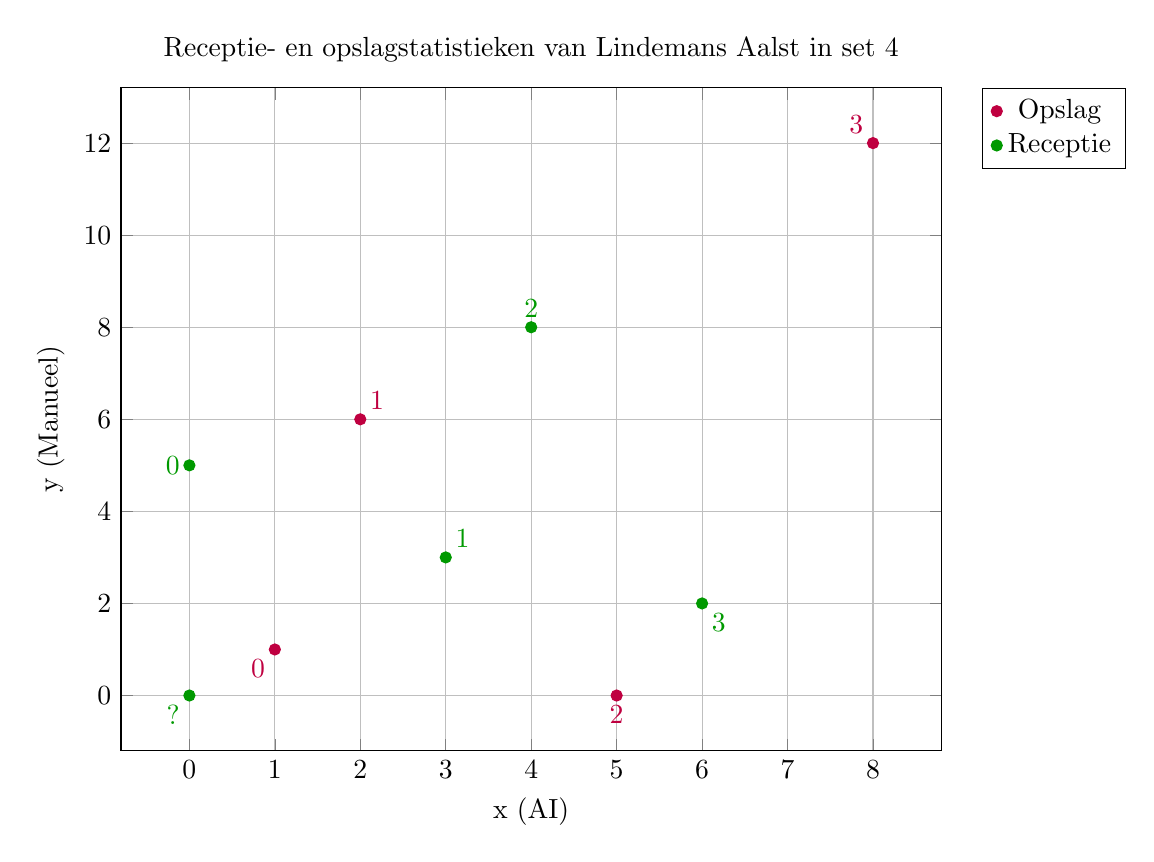
\begin{tikzpicture}
  \begin{axis}[
    title={Receptie- en opslagstatistieken van Lindemans Aalst in set 4},
    xlabel={x (AI)},
    ylabel={y (Manueel)},
    grid=major,
    legend style={at={(1.05,1)}, anchor=north west},
    width=12cm,
    height=10cm,
    enlargelimits=0.1,
  ]

  % Opslag
  \addplot[
    only marks,
    mark=*,
    color=purple,
  ] table {
    x y
    1 1
    2 6
    5 0
    8 12
  };
  \addlegendentry{Opslag}

  % Labels opslag
  \node at (axis cs:1,1) [anchor=north east, purple] {0};
  \node at (axis cs:2,6) [anchor=south west, purple] {1};
  \node at (axis cs:5,0) [anchor=north, purple] {2};
  \node at (axis cs:8,12) [anchor=south east, purple] {3};

  % Receptie
  \addplot[
    only marks,
    mark=*,
    color=green!60!black,
  ] table {
    x y
    6 2
    4 8
    3 3
    0 5
    0 0
  };
  \addlegendentry{Receptie}

  % Labels receptie
  \node at (axis cs:6,2) [anchor=north west, green!60!black] {3};
  \node at (axis cs:4,8) [anchor=south, green!60!black] {2};
  \node at (axis cs:3,3) [anchor=south west, green!60!black] {1};
  \node at (axis cs:0,5) [anchor=east, green!60!black] {0};
  \node at (axis cs:0,0) [anchor=north east, green!60!black] {?};

  \end{axis}
\end{tikzpicture}
\caption{AI invoer versus manuele invoer, ingedeeld in opslag en receptie, voor Lindemans Aalst in set 4.}
\label{fig:PL3ServeReceiveAalst4}
\end{figure}

In tabel \ref{tab:PL3SetAalstMan4} en \ref{tab:PL3DigAalstMan4} zijn de manueel ingevoerde spelverdelings- en verdedigingsstatistieken weergegeven. De statistieken van de AI zijn weergegeven in tabel \ref{tab:PL3SetDigAalstAI4}.
Bij de spelverdelingsstatistieken valt op dat Max Schulz een actie meer heeft bij de AI-invoer dan bij de manuele invoer. Bij het bekijken van de video valt dan wel op dat hij effectief een actie meer heeft uitgevoerd. 

Bij de verdedigingsstatistieken zijn er verschillende hoeveelheden. Bij 2 van de spelers is het wel correct. Bij de andere is er een verschil van 2 tot 1 actie minder door de AI-invoer.

\begin{table}[ht!]
    \centering
    \scriptsize
    \begin{tabular}{|l|c|c|c|c|c|c|c|c|}
        \hline
        \textbf{Speler} & *E\% & Tot & = & / & - & ! & + & \# \\ \hline
        Bert Dufraing & 100\% & 1 &  &  &  & & 1 &  \\ 
        Max Schulz & 100\% & 1 &  &  &  & & & 1 \\ 
        Lucas Lorente Lòpez & 100\% & 16 &  &  &  &  & 15 & 1 \\ 
        Matis Verwimp &100\% & 1 & & & & & 1 & \\\hline
    \end{tabular}
    \caption[Manueel ingevoerde spelverdelingsstatistieken voor Lindemans Aalst in set 4]{\label{tab:PL3SetAalstMan4}Manueel ingevoerde spelverdelingsstatistieken voor Lindemans Aalst in set 4.}
\end{table}

\begin{table}[ht!]
    \centering
    \scriptsize
    \begin{tabular}{|l|c|c|c|c|c|c|c|c|}
        \hline
        \textbf{Speler} & *E\% & Tot & = & / & - & ! & + & \# \\ \hline
        Bert Dufraing & 50\% & 2 &  & 1 & 1 &  &  & \\ 
        Berre Peters & 50\% & 4 & 1 & 1 & 1 & & 1 &  \\ 
        Max Schulz & 0\% & 1 & 1 &  &  &  &  & \\ 
        Nezar Harouk & 0\% & 1 &  &  & 1 &  &  &  \\ 
        Lucas Lorente Lòpez & 0\% & 1 &  &  & 1 &  &  & \\ \hline
    \end{tabular}
    \caption[Manueel ingevoerde verdedigingsstatistieken voor Lindemans Aalst in set 4]{\label{tab:PL3DigAalstMan4}Manueel ingevoerde verdedigingsstatistieken voor Lindemans Aalst in set 4.}
\end{table}

\begin{table}[ht!]
  \centering
  \scriptsize
  \begin{tabular}{|l|c|c|c|c|c|c|c|} \hline
    \textbf{Speler} & Ast & TA & SE & PCT & DS &  DE \\ \hline
    Bert Dufraing &  & 1 &  & 0\% & 1 &  \\
    Berre Peters &   &   &   &   & 2 &   \\
    Max Schulz &  & 2 &  & 0\% &   &   \\
    Nezar Harouk &   &   &   &   &  1 &   \\
    Lucas Lorente Lòpez & 10 & 16 &  & 62\% & 1 &  \\
    Matis Verwimp &  & 1 & & 0\% &   &   \\ \hline
  \end{tabular}
 \caption[Spelverdelings- en verdedigingsstatistieken gemaakt door Balltime AI voor Lindemans Aalst in set 4]{\label{tab:PL3SetDigAalstAI4}Spelverdelings- en verdedigingsstatistieken gemaakt door Balltime AI voor Lindemans Aalst in set 4.}
\end{table}

De aanvalsstatistieken in deze set worden weergegeven in de tabellen \ref{tab:PL3AttAalstMan4} en \ref{tab:PL3AttBlockAalstAI4}. De blokstatistieken zijn weergegeven in de tabellen \ref{tab:PL3BlockAalstMan4} en \ref{tab:PL3AttBlockAalstAI4}. De AI-invoer geeft aan dat Lucas Lorente Lòpez ook één keer aanvalt, terwijl de manuele invoer dit niet aangeeft. Bij het bekijken van de video is duidelijk dat hij dit effectief niet doet. De hoeveelheid correcte aanvallen is bij beide hetzelfde aantal.

Bij de blokstatistieken is er een zeer groot verschil aanwezig. De AI geeft aan dat er maar één blok doorheen de hele set is, terwijl de manuele invoer er negen in totaal aangeeft.

De kwaliteit van aanvallen en blokkeringen worden niet beoordeeld door de AI. 

\begin{table}[ht!]
    \centering
    \scriptsize
    \begin{tabular}{|l|c|c|c|c|c|c|c|c|}
        \hline
        \textbf{Speler} & *E\% & Tot & = & / & - & ! & + & \# \\ \hline
        Berre Peters & 43\% & 7 & 1 &  &  & & 2 & 4 \\ 
        Max Schulz & 20\% & 5 & 1 &  & 1 & 1 & & 2 \\ 
        Mihkel Varblane & -100\% & 1 &  & 1 &  &  &  & \\ 
        Alvaro Gimeno Rubio & 43\% & 7 &  & 1 & & & 2 & 4 \\ \hline
    \end{tabular}
    \caption[Manueel ingevoerde aanvalsstatistieken voor Lindemans Aalst in set 4]{\label{tab:PL3AttAalstMan4}Manueel ingevoerde aanvalsstatistieken voor Lindemans Aalst in set 4.}
\end{table}

\begin{table}[ht!]
    \centering
    \scriptsize
    \begin{tabular}{|l|c|c|c|c|c|c|c|c|}
        \hline
        \textbf{Speler} & *E\% & Tot & = & / & - & ! & + & \# \\ \hline
        Max Schulz & -100\% & 1 & 1 &  &  &  &  & \\
        Nezar Harouk & -75\% & 4 & 3 & &  & 1 &  & \\ 
        Mihkel Varblane & -33\% & 3 & 2 &  &  & &  & 1 \\ 
        Alvaro Gimeno Rubio & -100\% & 1 & 1 &  &  &  &  & \\  \hline
    \end{tabular}
    \caption[Manueel ingevoerde blokstatistieken voor Lindemans Aalst in set 4]{\label{tab:PL3BlockAalstMan4}Manueel ingevoerde blokstatistieken voor Lindemans Aalst in set 4.}
\end{table}

\begin{table}[ht!]
  \centering
  \scriptsize
  \begin{tabular}{|l|c|c|c|c|c|c|c|c|c|c|c|} \hline
    \textbf{Speler} &  K & E & TA & Atk\% & Kill\% & Error\% & BS & BA & BE \\ \hline
    Berre Peters & 4 & 1 & 7 & 0.43 & 57\% & 14\% &  &  & \\
    Max Schulz & 2 & 1 & 5 & 0.20 & 40\% & 20\% &  &  & \\
    Mihkel Varblane &  & 1 & 1 & -1.00 & 0\% & 100\% & 1 & & \\
    Alvaro Gimeno Rubio & 4 & 1 & 7 & 0.43 & 57\% & 14\% &  &  & \\
    Lucas Lorente Lòpez &  &  & 1 & 0 & 0\% & 0\% &  &  &\\ \hline
  \end{tabular}
  \caption[Aanvals- en blokstatistieken gemaakt door Balltime AI voor Lindemans Aalst in set 4]{\label{tab:PL3AttBlockAalstAI4}Aanvals- en blokstatistieken gemaakt door Balltime AI voor Lindemans Aalst in set 4.}
\end{table}
